\documentclass[a4paper, 12pt]{article}

\usepackage{cmap}
\usepackage[OT1]{fontenc}
\usepackage[utf8]{inputenc}
%\usepackage{mathtext}
%\usepackage{amsmath}
\usepackage[russian]{babel}
\usepackage{amsmath}
\usepackage{amsfonts}
\usepackage{amssymb}
\usepackage{graphicx}
%\usepackage[bookmarks=true, pdfpagemode=UseNone]{hyperref}
\usepackage{indentfirst}
\usepackage{listings}
%\usepackage{multicol}
%\usepackage{misccorr}
%\usepackage{longtable}
%\usepackage{flafter}
\usepackage{float}
%\usepackage{color}
%\usepackage{nccfloats}
%\usepackage{tabularx}
%\usepackage{graphicx}
%\usepackage[babel=true,protrusion=true,expansion=true]{microtype}
%\usepackage[left=1.8cm, right=1cm, top=1cm, bottom=1cm, bindingoffset=0cm]{geometry}

%\pagestyle{empty}

\author{Алексюк А.О., Мурашко Д.С.}
\title{Визуализация сигналов во временной и частотной области}
\lstset{inputencoding=utf8, extendedchars=\true, keepspaces = true, language=Matlab}

\begin{document}
\maketitle
\tableofcontents
\pagebreak

\section{Цель работы}
Познакомиться со средствами генерации сигналов и визуализации их спектров.

\section{Постановка задачи}
В командном окне MATLAB и в среде Simulink промоделировать чистый синусоидальный сигнал, а также синусоидальный сигнал с шумом. Получить их спектры.

\section{Теоретическая часть}

Преобразование Фурье в интегральной форме:

$$\hat{f}(\omega)=\frac{1}{\sqrt{2\pi}}\int\limits_{-\infty}^{\infty}f(x)e^{-ix\omega}\,dx$$

Дискретное преобразование Фурье:

$$X_k = \sum_{n=0}^{N-1} x_n e^{-\frac{2 \pi i}{N} k n} \qquad k = 0, \dots, N-1$$

Обратное преобразование:

$$x_n = \frac{1}{N} \sum_{k=0}^{N-1} X_k e^{\frac{2\pi i}{N} k n} \quad \quad n = 0,\dots,N-1.$$

\section{Ход работы}

\subsection{Код Matlab}
\begin{lstlisting}
close all;
clear all;
x = 0:0.01:4*pi;
f0 = 5;
%исходный сигнал
y = sin(2*pi*f0*x);
plot(x(1:200),y(1:200))
grid
%спектр исходного сигнала 
figure
spectrum = abs(fft(y,128)); 
norm_spectrum = spectrum.*conj(spectrum)/512;
f=100*(0:127)/512;
plot(f, norm_spectrum(1:128))
axis([0 max(f) 0 10])
grid
\end{lstlisting}

\begin{figure}[H]
   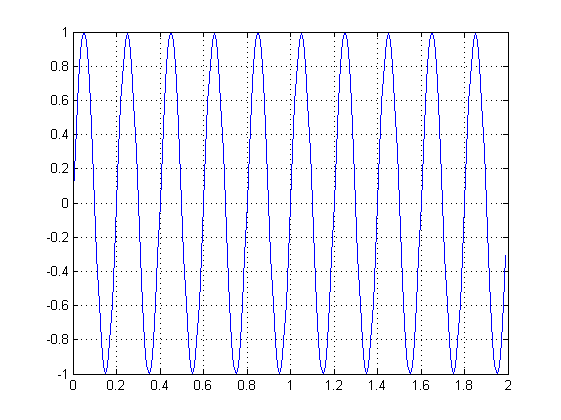
\includegraphics[scale=0.7]{lab4/sin.png}
   \caption{Синусоида}
\end{figure}

\begin{figure}[H]
   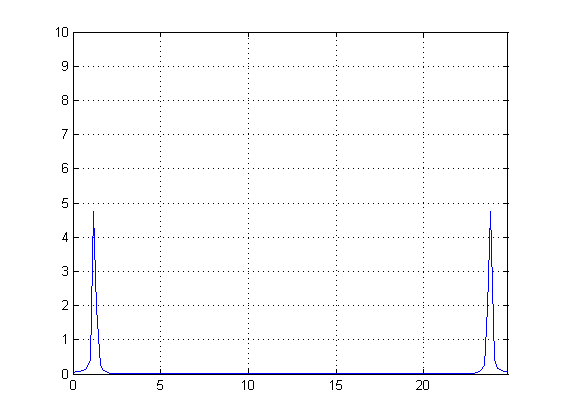
\includegraphics[scale=0.7]{lab4/spectre.png}
   \caption{Спектр}
\end{figure}

\subsection{Simulink}

\begin{figure}[H]
   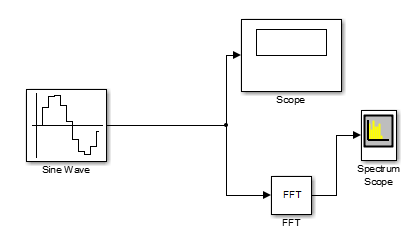
\includegraphics[scale=0.7]{lab4/simulink.png}
   \caption{Проект Simulink}
\end{figure}

\begin{figure}[H]
   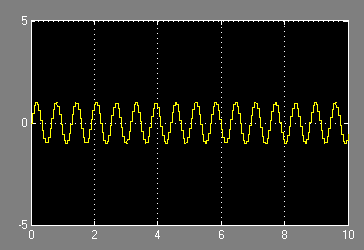
\includegraphics[scale=0.7]{lab4/sin_simulink.png}
   \caption{Синус}
\end{figure}

\begin{figure}[H]
   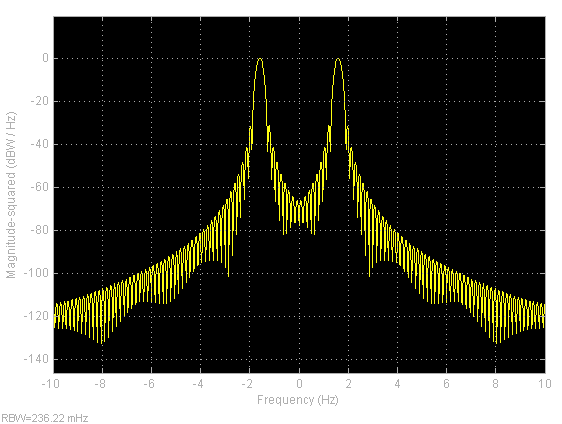
\includegraphics[scale=0.7]{lab4/scope.png}
   \caption{Спектр}
\end{figure}

\section{Вывод}

В ходе работы были исследованы два важных нюанса, касающиеся применения преобразования Фурье в цифровых системах.

Во-первых, если бы входной сигнал был бесконечным, то его спектр представлял бы собой бесконечно короткий импульс, с бесконечно большой амплитудой и единичной площадью, однако на практике из-за ограниченной длины сигнала (бесконечный сигнал был как бы умножен на прямоугольный импульс конечной длины) произошла свертка с дельта-импульсом.

Во-вторых, так как сигнал был дискретизирован, то импульс повторяется бесконечное число раз с периодом равным частоте дискретизации (на графике видно два импульса).

\end{document}